\section{Module 3. Non-stationary noise estimation}
In order to test effectiveness of implemented algorithm the results of it were compared to results of algorithm prepared to perforem calculatioans contained in \cite{aja2015spatially}. The algorithm for the article was implemented in Matlab.
\begin{figure}[H]
	\centering{}
		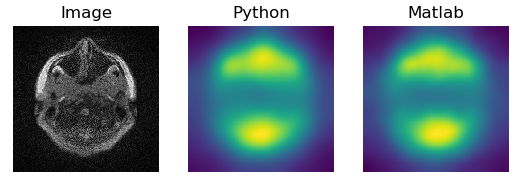
\includegraphics[scale=0.7]{figures/module03/10_comp}
	\caption{Image (left), noise map form Python algorithm(middle), noise map form Matlab algorithm(right).} 
\end{figure}
\begin{figure}[H]
	\centering{}
		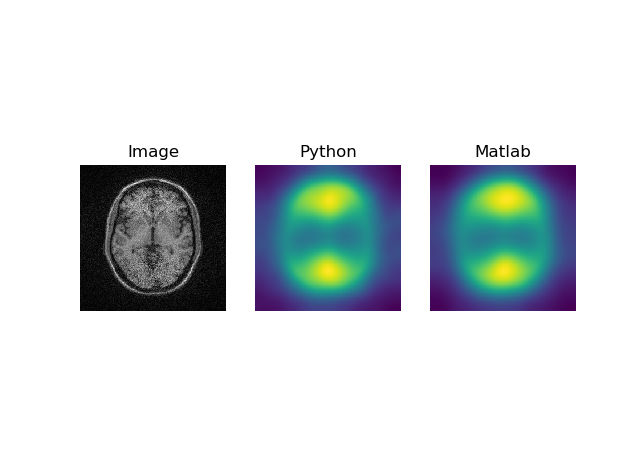
\includegraphics[scale=0.7]{figures/module03/70_comp}
	\caption{Image (left), noise map form Python algorithm(middle), noise map form Matlab algorithm(right).} 
\end{figure}
\begin{figure}[H]
	\centering{}
		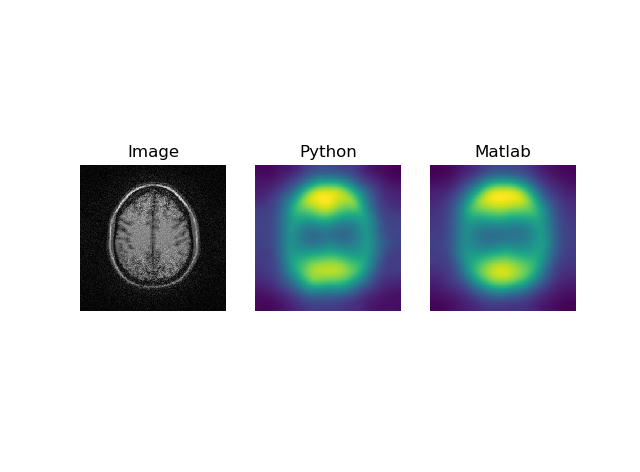
\includegraphics[scale=0.7]{figures/module03/110_comp}
	\caption{Image (left), noise map form Python algorithm(middle), noise map form Matlab algorithm(right).} 
\end{figure}
\begin{figure}[H]
	\centering{}
		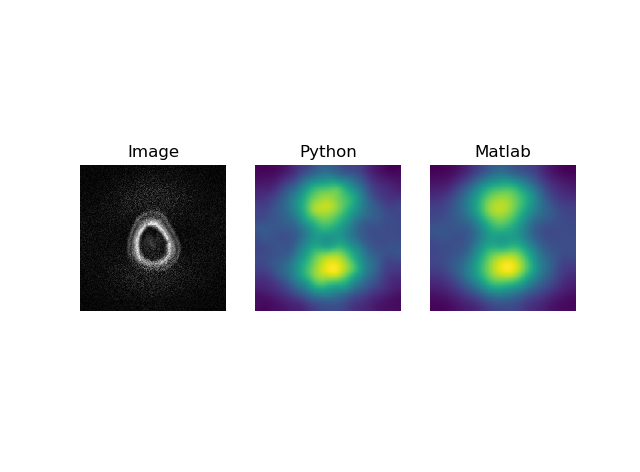
\includegraphics[scale=0.7]{figures/module03/160_comp}
	\caption{Image (left), noise map form Python algorithm(middle), noise map form Matlab algorithm(right).} 
\end{figure}
Results from Python algorithm are not perfect equivalent of the results from Matlab algorithm however ther are very similar and seem to be suitable for 
further processing of the image.